\documentclass{beamer}
\usepackage[utf8]{inputenc}

\usetheme{Madrid}
\usecolortheme{default}
\usepackage{amsmath,amssymb,amsfonts,amsthm}
\usepackage{txfonts}
\usepackage{tkz-euclide}
\usepackage{listings}
\usepackage{adjustbox}
\usepackage{array}
\usepackage{tabularx}
\usepackage{gvv}
\usepackage{lmodern}
\usepackage{circuitikz}
\usepackage{tikz}
\usepackage{graphicx}

\setbeamertemplate{page number in head/foot}[totalframenumber]

\usepackage{tcolorbox}
\tcbuselibrary{minted,breakable,xparse,skins}



\definecolor{bg}{gray}{0.95}
\DeclareTCBListing{mintedbox}{O{}m!O{}}{%
  breakable=true,
  listing engine=minted,
  listing only,
  minted language=#2,
  minted style=default,
  minted options={%
    linenos,
    gobble=0,
    breaklines=true,
    breakafter=,,
    fontsize=\small,
    numbersep=8pt,
    #1},
  boxsep=0pt,
  left skip=0pt,
  right skip=0pt,
  left=25pt,
  right=0pt,
  top=3pt,
  bottom=3pt,
  arc=5pt,
  leftrule=0pt,
  rightrule=0pt,
  bottomrule=2pt,

  colback=bg,
  colframe=orange!70,
  enhanced,
  overlay={%
    \begin{tcbclipinterior}
    \fill[orange!20!white] (frame.south west) rectangle ([xshift=20pt]frame.north west);
    \end{tcbclipinterior}},
  #3,
}
\lstset{
    language=C,
    basicstyle=\ttfamily\small,
    keywordstyle=\color{blue},
    stringstyle=\color{orange},
    commentstyle=\color{green!60!black},
    numbers=left,
    numberstyle=\tiny\color{gray},
    breaklines=true,
    showstringspaces=false,
}
%------------------------------------------------------------
%This block of code defines the information to appear in the
%Title page
\title %optional
{5.3.25}
\date{\today}
%\subtitle{A short story}

\author % (optional)
{Shivam Sawarkar \\ AI25BTECH11031}



\begin{document}


\frame{\titlepage}
\begin{frame}{Question}
    Solve the following pair of linear equations
\begin{align}
3x + 4y = 10
\end{align}
\begin{align}
2x - 2y = 2
\end{align}
\end{frame}

\begin{frame}{Solution}
    Given equations:
\begin{align}
\myvec{3 & 4}\Vec{x}=10
\end{align}
\begin{align}
\myvec{2 & -2}\Vec{x}=2
\end{align}

In augmented matrix form:
\begin{align}
\augvec{2}{1}{3 & 4 & 10 \\ 2 & -2 & 2}
\end{align}
\end{frame}

\begin{frame}{Solution}
    \begin{align}
R_2 \rightarrow R_2 - \tfrac{2}{3}R_1
\Rightarrow
\augvec{2}{1}{
3 & 4 & 10 \\
0 & -\tfrac{14}{3} & -\tfrac{14}{3}
}
\end{align}

\begin{align}
R_2 \rightarrow -\tfrac{3}{14}R_2
\Rightarrow
\augvec{2}{1}{
3 & 4 & 10 \\
0 & 1 & 1
}
\end{align}

\begin{align}
R_1 \rightarrow R_1 - 4R_2
\Rightarrow
\augvec{2}{1}{
3 & 0 & 6 \\
0 & 1 & 1
}
\end{align}

\begin{align}
R_1 \rightarrow \tfrac{1}{3}R_1
\Rightarrow
\augvec{2}{1}{
1 & 0 & 2 \\
0 & 1 & 1
}
\end{align}

Hence,
\begin{align}
x = 2, \quad y = 1.
\end{align}
\end{frame}

\begin{frame}{Plot}
    \begin{figure}
        \centering
        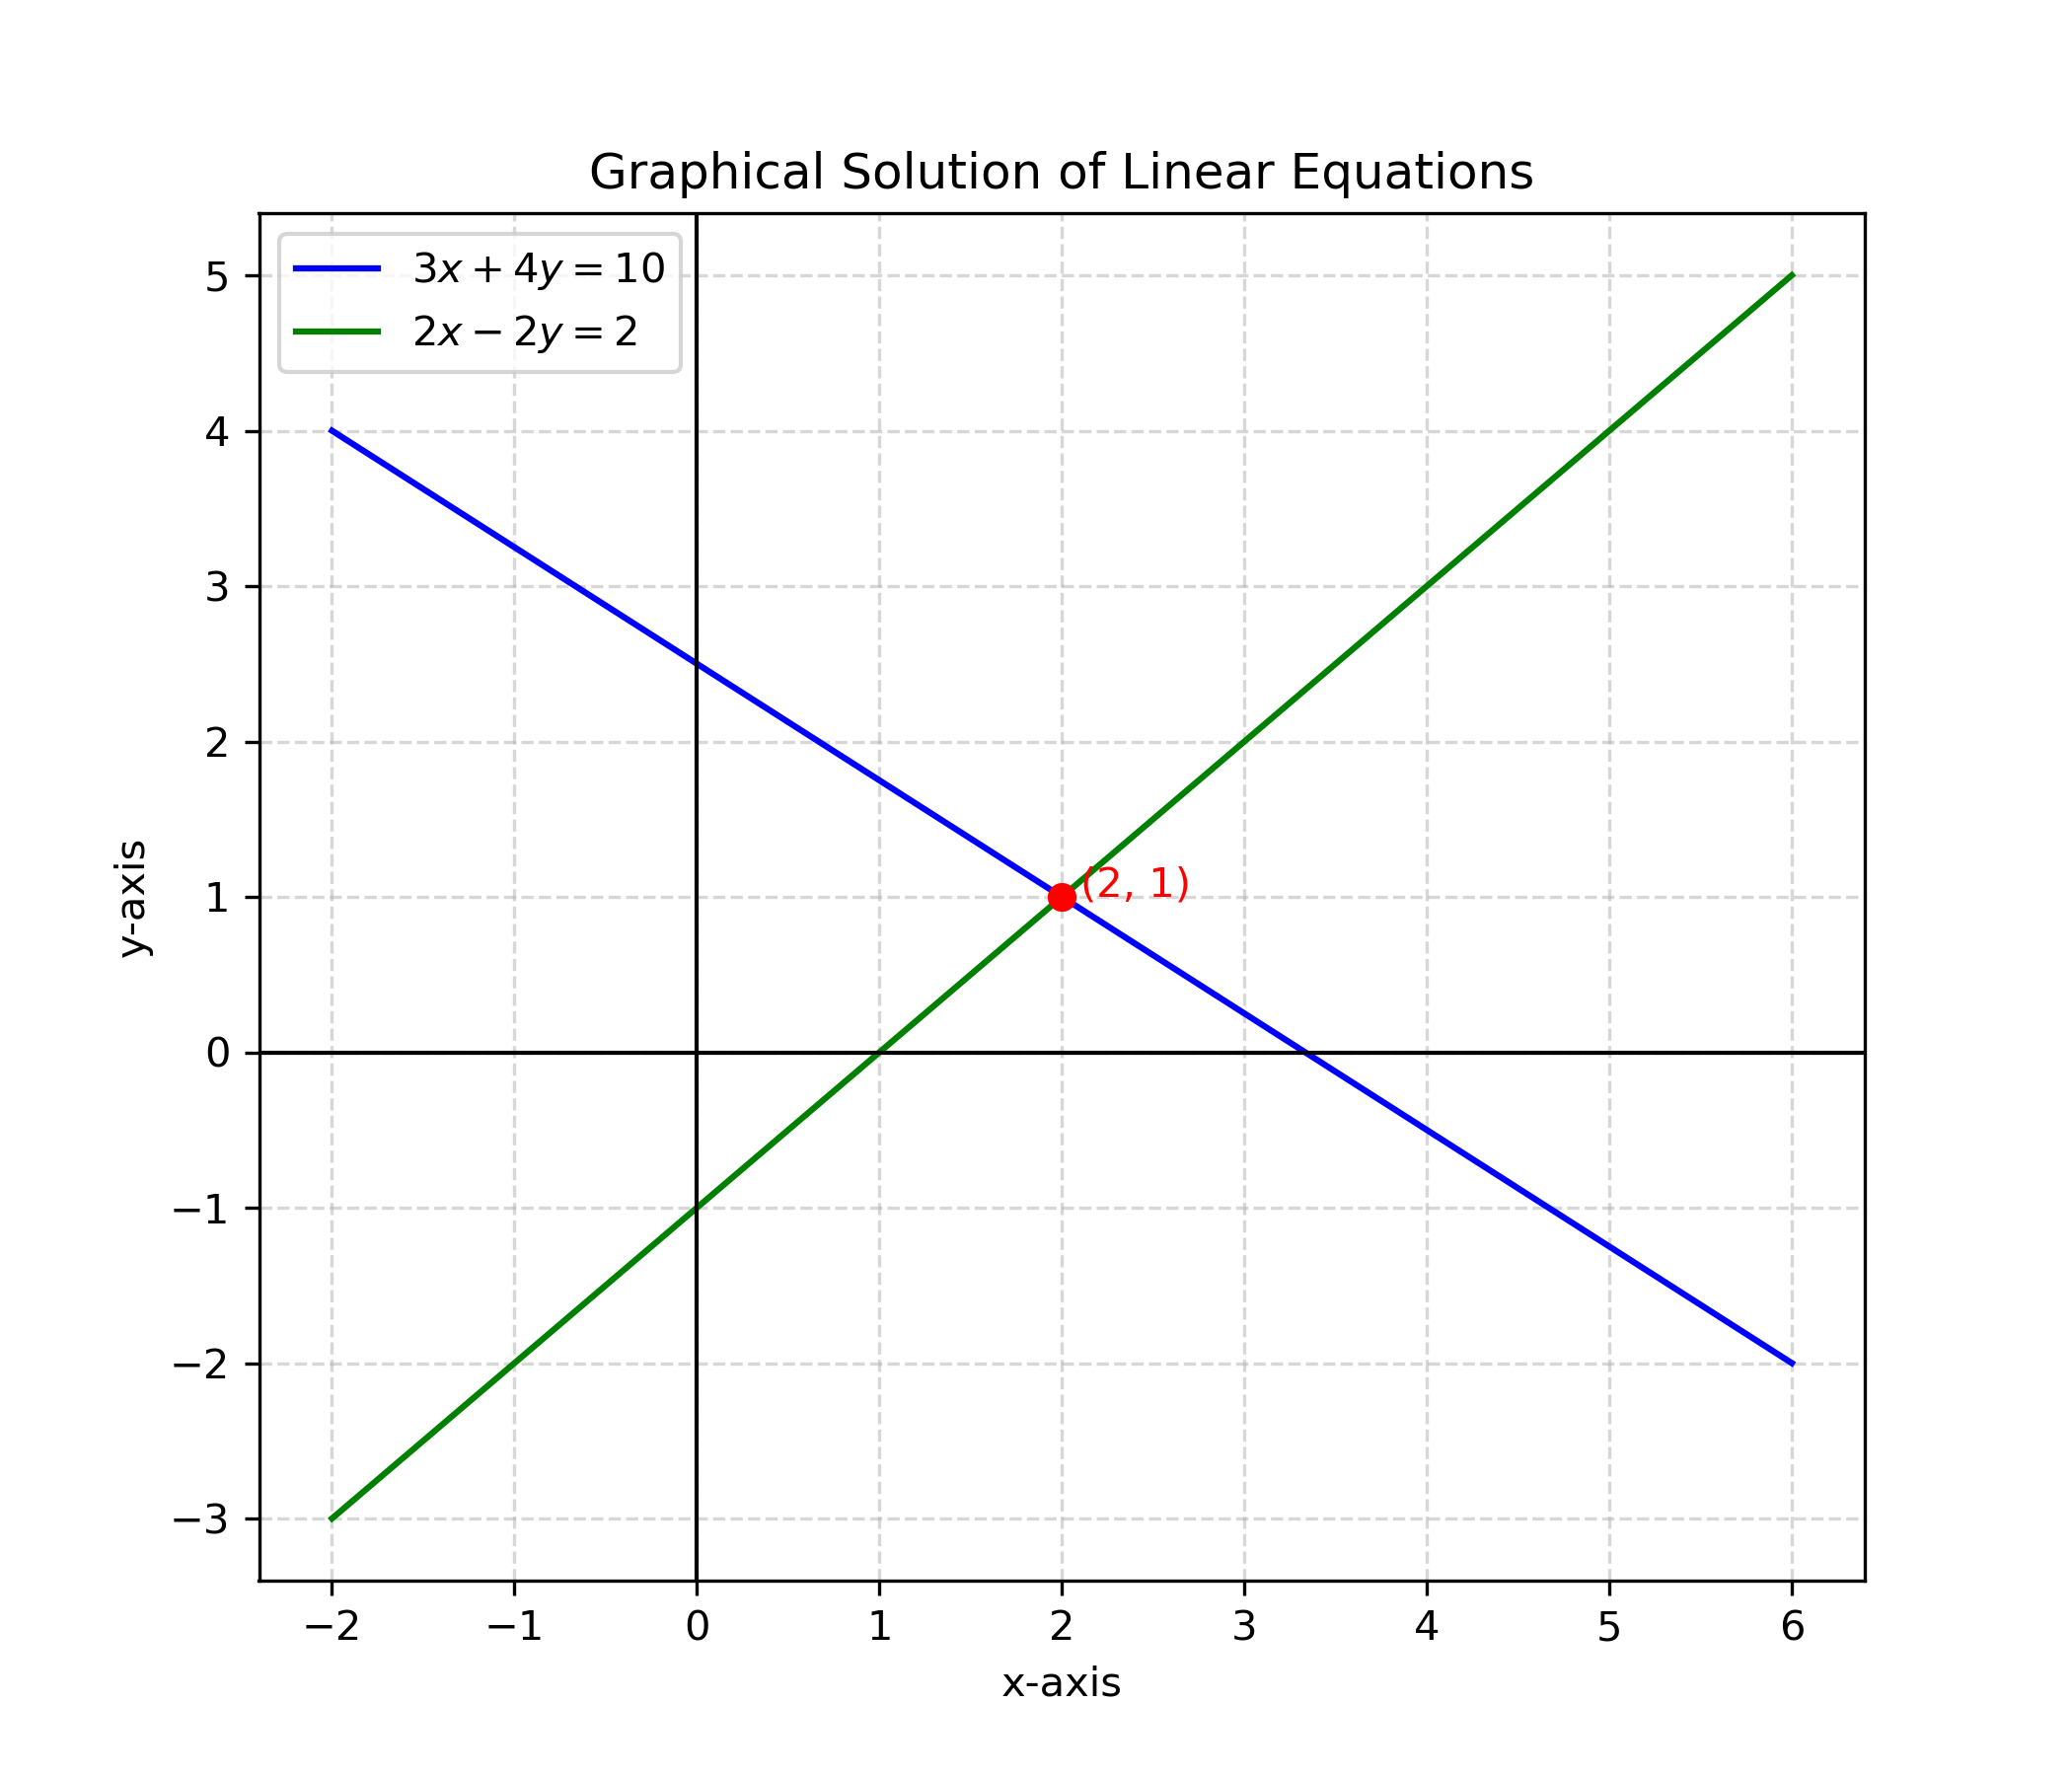
\includegraphics[width=0.8
        \linewidth]{figs/plot11.png}
        \caption{}
        \label{fig:placeholder}
    \end{figure}
\end{frame}

\begin{frame}[fragile]{C Code}
    \begin{verbatim}
#ifndef LINEAR_H
#define LINEAR_H

#include <stdio.h>

// Function to take input for coefficients
void input_equations(float *a1, float *b1, float *c1, float *a2, float *b2, float *c2) {
    printf("Enter coefficients of first equation (a1 b1 c1): ");
    scanf("%f %f %f", a1, b1, c1);
    printf("Enter coefficients of second equation (a2 b2 c2): ");
    scanf("%f %f %f", a2, b2, c2);
}

// Function to compute determinant
float determinant(float a1, float b1, float a2, float b2) {
    return (a1 * b2) - (a2 * b1);
}
    \end{verbatim}
\end{frame}

\begin{frame}[fragile]{C Code}
    \begin{verbatim}
// Function to solve equations
void solve_equations(float a1, float b1, float c1, float a2, float b2, float c2) {
    float det = determinant(a1, b1, a2, b2);

    if (det == 0) {
        printf("The equations have no unique solution (parallel or coincident lines).\n");
    } else {
        float x = (c1 * b2 - c2 * b1) / det;
        float y = (a1 * c2 - a2 * c1) / det;
        printf("Solution: x = %.2f, y = %.2f\n", x, y);
    }
}

#endif
    \end{verbatim}
\end{frame}

\begin{frame}[fragile]{C Code}
    \begin{verbatim}
#include "solution.h"

int main() {
    float a1, b1, c1, a2, b2, c2;

    // Input the equations
    input_equations(&a1, &b1, &c1, &a2, &b2, &c2);

    // Solve the equations
    solve_equations(a1, b1, c1, a2, b2, c2);

    return 0;
}
    \end{verbatim}
\end{frame}

\begin{frame}[fragile]{Python Code}
    \begin{verbatim}
def determinant(a1, b1, a2, b2):
    """Compute the determinant of coefficient matrix"""
    return a1 * b2 - a2 * b1

def solve_equations(a1, b1, c1, a2, b2, c2):
    """Solve the two equations using Cramer's Rule"""
    det = determinant(a1, b1, a2, b2)

    if det == 0:
        print("The equations have no unique solution (parallel or coincident lines).")
    else:
        x = (c1 * b2 - c2 * b1) / det
        y = (a1 * c2 - a2 * c1) / det
        print(f"Solution: x = {x:.2f}, y = {y:.2f}")
    \end{verbatim}
\end{frame}

\begin{frame}[fragile]{Python Code}
    \begin{verbatim}
def main():
    print("Enter coefficients for the equations:")
    a1, b1, c1 = map(float, input("a1 b1 c1: ").split())
    a2, b2, c2 = map(float, input("a2 b2 c2: ").split())

    solve_equations(a1, b1, c1, a2, b2, c2)

if __name__ == "__main__":
    main()
    \end{verbatim}
\end{frame}

\begin{frame}[fragile]{Python + C Code}
    \begin{verbatim}
import ctypes

# Load the shared library
lib = ctypes.CDLL('./solution.so')

# Define argument and return types for solve_equations
lib.solve_equations.argtypes = [ctypes.c_float, ctypes.c_float, ctypes.c_float,
                                ctypes.c_float, ctypes.c_float, ctypes.c_float]
lib.solve_equations.restype = None

# Python wrapper function
def solve_from_c(a1, b1, c1, a2, b2, c2):
    lib.solve_equations(a1, b1, c1, a2, b2, c2)
    \end{verbatim}
\end{frame}

\begin{frame}[fragile]{Python + C Code}
    \begin{verbatim}
# Take user input
print("Enter coefficients of first equation (a1 b1 c1): ")
a1, b1, c1 = map(float, input().split())

print("Enter coefficients of second equation (a2 b2 c2): ")
a2, b2, c2 = map(float, input().split())

# Call the C function
solve_from_c(a1, b1, c1, a2, b2, c2)
    \end{verbatim}
\end{frame}








\end{document}